% !TeX root = ../index.tex

\section{Einleitung}\label{sec:einleitung}

Dieser Bericht beschreibt eine Laborarbeit, welche im Rahmen der Vorlesung \enquote{W3M20018.1 Data Science \& Big Data} durchgeführt wurde.\footnote{\href{https://farberg.de/talks/big-data/?01\%20-\%20Introduction.md\#/2}{https://farberg.de/talks/big-data/?01 - Introduction.md\#/2}}
Gegenstand der Laborarbeit ist die Abwandlung eines vorgegebenen Big Data Setups, um damit einen eigens ausgewählten Use Case abzubilden.\footnote{\href{https://farberg.de/talks/big-data/?06\%20-\%20Use\%20Case.md\#/}{https://farberg.de/talks/big-data/?06 - Use Case.md\#/}}
Die praktischen Ergebnisse der Arbeit sind im GitHub Repository \href{https://github.com/kevinsieverding/dhbw-w3m200181-app}{kevinsieverding/dhbw-w3m200181-app} zu finden.
Im Folgenden beschreibt Abschnitt \ref{sec:use-case} den gewählten Use Case, Abschnitt \ref{sec:architektur} die gewählte Architektur und Umsetzung bevor Abschnitt \ref{sec:fazit} ein Fazit darlegt.

\section{Use Case}\label{sec:use-case}

Das originale Setup stellt eine Reihe von Artikeln über einen Web-Server bereit, zeichnet Seitenaufrufe auf und schreibt sie in Kafka, von wo sie ein Spark Job aufnimmt und aggregiert, um Popularitätsstatistiken zu erstellen, welche wiederum auf der Web-Seite angezeigt werden.
Der Use Case befasst sich also mit einer simplen Analyse von Nutzerverhalten.

\subsection{Brainstorming}

Um einen geeigneten Use Case zu wählen, habe ich zunächst ein Brainstorming betrieben, bis ich eine zufriedenstellende Idee entwickelt hatte.
Im Folgenden möchte ich gerne einige meiner verworfenen Ideen vorstellen, bevor ich den von mir letztendlich gewählten Use Case näher beschreibe.

\subsubsection{Warenkorbanalyse mittels Apriori Algorithmus}

Mein erster Gedanke war, in bei der Nutzeranalyse zu bleiben und eine andere Form der Analyse zu implementieren.
Da ich in meiner Arbeit als Entwickler bei der SAP im Bereich Standardsoftware für den Einkauf mit internen Bestellplatformen zu tun habe, überlegte ich eine simple Warenkorbanalyse mittels des \enquote{Apriori} Algorithmus zu implementieren.
\parencite{agrawal_fast_1994}

Hierzu würde ich einen simplen Web-Shop implementieren, welcher dem Nutzer einen Katalog von Produkten anzeigt, welche dieser in seinen Warenkorb legen und bestellen kann.
Die Bestellungen mitsamt der Positionen würden in Kafka geschrieben werden, wo ein Spark Job den Apriori Algorithmus anwendet, um Tupel von häufig zusammen gekauften Produkten zu identifizieren.
Diese Information würde der Spark Job in eine MariaDB Datenbank persistieren, wo sie von der Web-App abgefragt werden könnte, um dem Nutzer einen Vorschlag wie \enquote{Kunden kauften ebenfalls:  \ldots} anzuzeigen, wie man ihn von den Webseiten von vielen großen Online-Händlern kennt.

Letzenendes habe ich mich dagegen entschieden diesen Use Case so zu implementieren, weil mir der notwendige Aufwand als schwierig abzuschätzen und tendenziell groß erschien.
Die Implementierung des Web-Shops mit nicht-existenten Kenntnissen in der Web-Entwicklung, sowie die nicht trivial erscheinende Implementierung des Apriori Algorithmus in Spark waren dabei ausschlaggebend.
Aus diesem Grund habe ich mich nach einem Use Case umgeschaut, welcher in einem kleineren Rahmen umzusetzen sei.

\subsubsection{Analyse der Parksituation in Heidelberg}

Anschließend überlegte ich die Parksituation in meiner aktuellen Heimatstadt Heidelberg zu analysieren.
Die größte Herausforderung dabei schien mir, geeignete Daten zu finden.
Unter \url{https://parken.heidelberg.de/} bietet die Stadt Heidelberg bereits eine digitale Übersicht der aktuellen Parksituation an, woraus sich schließen lässt, dass diese Daten nicht nur bereits gesammelt und analysiert werden, sondern auch über das Internet zugreifbar sind.

Leider stellte sich bei einer oberflächlichen Analyse der Webseite heraus, dass die zugrundeliegende Daten-API nicht ohne Weiteres über andere Wege zugreifbar ist.
Während sich mit hoher Wahrscheinlichkeit ein Weg finden ließe, die API dennoch programmatisch auszulesen, so wollte ich die damit einhergehende Unsicherheit und den möglichen Aufwand für das Schreiben eines Clients/Crawlers für die API vermeiden.
Daher habe ich auch diese Option verworfen.

\subsection{Analyse von Messwerten zur Überwachung von Industriemaschinen}

Als drittes habe ich mich mit einem weiteren Umfeld auseinandergesetzt, in dem Big Data seit längerem eine große Rolle spielt: Predictive Maintenance.
\citeauthor{hashemian_state---art_2011} beschreibt moderne Predictive Maintenance wie folgt: \enquote{[A]utomated methods that use advanced signal processing techniques based on pattern recognition, including neural networks, fuzzy logic, and data-driven empirical and physical modeling.} \parencite{hashemian_state---art_2011}

Hier ließen sich verschiedene frei verfügbare Datensätze finden, welche als Basis für die Implementierung einer Big Data Anwendung dienen konnten.
Ich bin schließlich auf einen Datensatz der ZeMA gGmbH gestoßen, welcher im Rahmen von \cite{helwig_condition_2015} erstellt wurde und Daten von verschiedenen Sensoren eines hydraulischen Test-Systems enthält, die über mehrere Betriebszyklen hinweg aufgezeichnet wurden.\footnote{\url{https://archive.ics.uci.edu/ml/datasets/Condition+monitoring+of+hydraulic+systems}}

\begin{figure}[H]
  \centering
  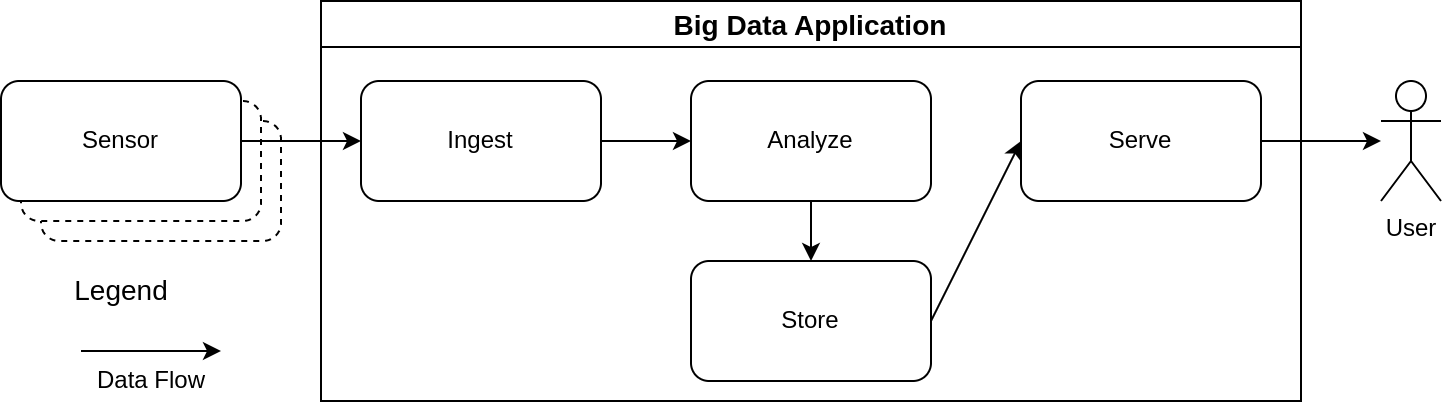
\includegraphics[width=0.9\textwidth]{use-case.drawio.png}
  \caption{Grobes Modell des gewählten Use Case}\label{fig:use-case}
\end{figure}

Auf Basis dieses Datensatzes definierte ich den Use Case, für den ich das Big Data Setup aufbauen wollte.
Abbildung \ref{fig:use-case} zeigt, wie zunächst Messwerte von einem oder mehreren Sensoren in die Applikation geladen werden sollen.
Diese Daten sollen analysiert und die erarbeiten Ergebnisse persistiert werden.
Persistierte Ergebnisse können anschließend Nutzern zur Verfügung gestellt werden.

\section{Architektur}\label{sec:architektur}

\begin{figure}[H]
  \centering
  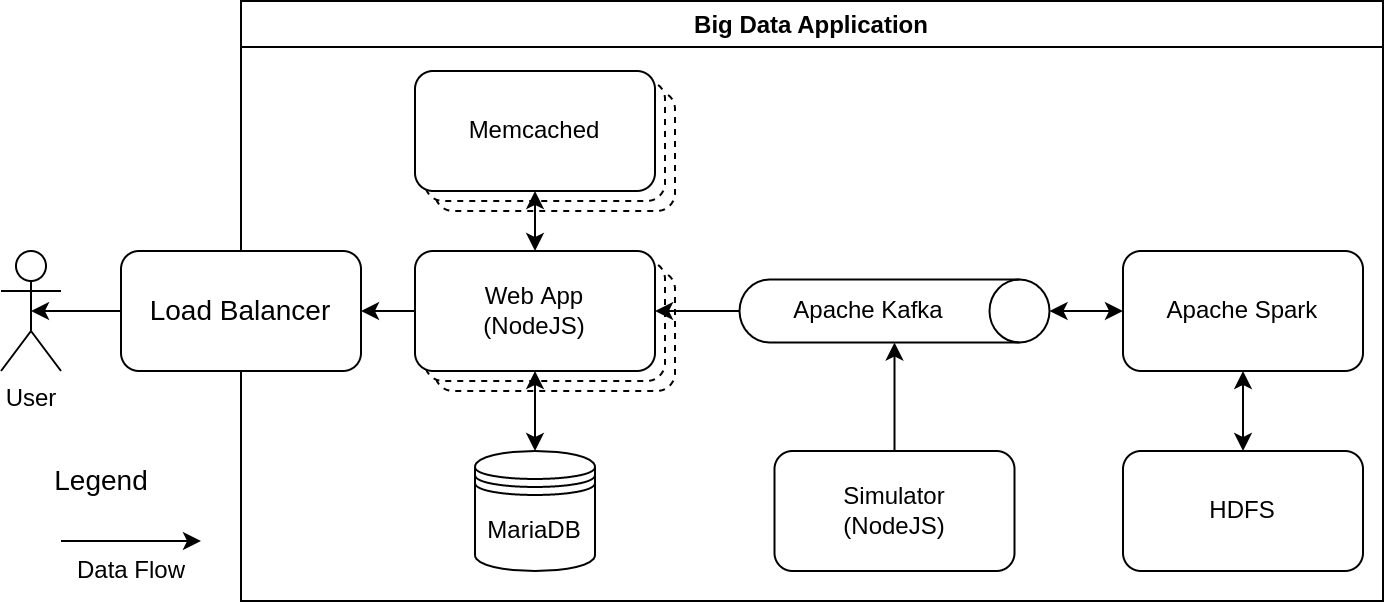
\includegraphics[width=0.9\textwidth]{architecture.drawio.png}
  \caption{Architektur der implementierten Big Data Anwendung}\label{fig:architektur}
\end{figure}

\section{Fazit}\label{sec:fazit}
